\chapter{Standard Model}

The standard model of particle physics is a theoretical model that describes
almost all sub-nuclear phenomena up to an energy scale of
$\mathcal{O}(\unit{100}{\GeV})$.

The theory was pieced togethere in the 60s and 70s and comprises two families of
elementary particles, called quarks and leptons, and incorporates the theories
of quantum electrodynamics (QED), Glashow-Weinberg-Salam theory of electroweak
dynamics and quantum chromodynamics (QCD).

The Standard Model is remarkable in its accuracy, describing every experimental
test performed.  
The chapter will first introduce the two families of elementary matter
particles, the leptons and quarks, and then summarize the theoretical background
to the standard model.

\section{Constituents of the Standard Model}
Within the Standard Model matter is described as being constructed from a small
number of spin$=\nicefrac{1}{2}$ particles called fermions that interact with
the electromagnetic, weak and strong forces. The fermions are divided in to two
families called, leptons and quarks, according to their experimentally measured
properties such as their charge. Each fermion varies in mass from the light
neutrinos (\todo{neutrino mass here}) to the heavy top quark (\todo{top mass
here}).

Each family of fermions can be further subdivided in to three generations that
increase progressivly increase in mass. The fermions of the Standard Model and
some of their properties are sumarised in \TableRef{tab:particles}.

\begin{table}
\begin{center}
\begin{tabular}{ l l l l l l }
& 1st gen. & 2nd gen. & 3rd gen. & $Q$ & colour \\ \hline
\multirow{2}{*}{quarks} 
& \Pup   & \Pstrange & \Ptop & $\nicefrac{+2}{3}$ & \multirow{2}{*}{RGB} \\
& \Pdown & \Pcharm   & \Pbottom & $\nicefrac{+2}{3}$ & \\ \hline
\multirow{2}{*}{leptons} 
& \Pnue      & \Pnum  & \Pnut & $0$ & \multirow{2}{*}{-} \\
& \Pelectron & \Pmuon & \Ptau & $1$ & \\ \hline
\end{tabular}
\caption{The fermions of the Standard Model.}
\end{center}
\label{tab:particles}
\end{table}\todo{add particle masses?}

Each lepton generation contains a charged lepton and a corresponding light
neutral particle called a neutrino. All leptons interact via the weak force
where as only the charge lepton interacts with the electromagnetic force.  The
first generation of leptons is the most familiar containing the electron and the
electron neutrino.

Unlike leptons, quarks carry fractional charge, within each generation there is
a quark with a charge of $\nicefrac{2}{3}$ and another with a charge of
$\nicefrac{-1}{3}$. As well as the electric charge, quarks carry an additional
charge called the colour charge. The colour charge allows the quarks to interact
via the strong force in addition the electromagnetic and the weak forces.
The first generation of quarks is again the most familiar, containing the up and
down type quarks that are the constituents of the proton and neutron, which in
turn, with the electron, form atoms and all familiar matter.

\todo[inline]{antiparticles}

The heavier generations of quarks (strange, charm, bottom and top, or \Pstrange,
\Pcharm, \Pbottom and \Ptop) are unstable and decay eventually to \Pup or
\Pdown.
The heavy leptons, muon (\Pmuon) and tau (\Ptau), decay in a similar manner to
the stable electron. 
Due to the instability of the heavier generations of fermions, they can only be
found in  cosmic rays, or produced in high energy physics experiments.

An important property of a fermion is the ``handedness'' or chirality. A left
handed particle has its spin aligned in the oposite direction to its direction
of motion and a right handed particle is one where the are both aligned

In the standard model, the strong, weak and electromagnetic interactions are
described as the exchange of integer spin intermediate particles called bosons.
The electromagnetic force is mediated by the massless, chargeless photon. The
strong force is mediated by eight massless gluons. 
The weak force is mediated by the exchage of massive particles, the \PWpm and \PZ
bosons. The \PWpm boson is unique in that it only interacts with left handed
particles.

\todo[inline]{more?}


\section{Theoretical Background}
This section will introduce some of the ideas that drive the
theoretical background to the Standard Model.

\subsection{Symmetry and Groups}
Noether's theorem states that for every symmetry of nature, there is
a corresponding quantity that is conserved and conversely each conservation law
is the result of some underlying symmetry.
\todo[inline]{this whole section is horrible}

For example, the laws of physics are symmetrical with respect to translations in
time ad space, and this leads directly to conservation of energy and momentum
respectivly. Other symmetries and conservation laws are summarised in
\TableRef{tab:symmetry}

\begin{table}
\begin{center}
\begin{tabular}{ l l }
Symmetry & Conserved Quantity \\ \hline
Time     & Energy \\
Space    & Momentum \\
Rotation & Angular Momentum \\
Gauge    & Electric Charge \\
\end{tabular}
\caption{Examples of symmetries and their corresponding conservation laws.}
\end{center}
\label{tab:symmetry}
\end{table}

It is currently believed that all particle interactions are dictated by symmetry
principles.  In group theory symmetry operations, such as rotations, can be
described by mathematical groups.
The most common groups to physics are unitary groups, $U(n)$, which are the
collection of all the $n\times n$ unitary ($U^{-1} = \tilde{U}^{*}$) matrices, and
the special unitary groups, $SU(n)$, which have the additional requirement that
the matrices have a determinant of 1.

\subsection{QED}
In QED an electron can be described as a complex field, $\psi$. The Lagrangian is
given by
\begin{equation}
\mathcal{L} = i \bar{\psi} \gamma_{\mu} \partial^{\mu} \psi - m \bar{\psi}\psi
\end{equation}
This Lagrangian is invariant under a `global' phase transformation
\begin{equation}
\psi(x) \to e^{i\alpha} \psi(x)
\label{eq:global}
\end{equation}
where $\alpha$ is a global arbitary parameter. The Lagrangian is said to exhibit
global gauge invariance. The family of transfomations, $R =
e^{i \alpha}$, where $\alpha$ is real and continuous, forms the unitary
abelian \footnote{Abelian refers to the property that all the elements in a
group commute, $R(\alpha)R(\beta) = R(\beta)R(\alpha)$.}
group $U(1)$. 
More generally, the \EquationRef{eq:global} can be rewritten as 
\begin{equation}
\psi(x) \to e^{i\alpha(x)} \psi(x)
\label{eq:local}
\end{equation}
where $\alpha$ is now a function of the space time coordinate $x$. This is known
as a local phase transformation. Unfortunately under this transformation the
Lagrangian is no longer invariant. This can be overcome by defining the
covariant derivative as 
\begin{equation}
D_{\mu} \equiv \partial_{\mu} - i e A_{\mu}
\end{equation}
where an aditional vector field $A_{\mu}$ has been added, that transforms as 
\begin{equation}
A_{\mu} \to A_{\mu} + \frac{1}{e} \partial_{\mu} \alpha
\end{equation}
and the new Lagrangian becomes
\begin{equation}
\mathcal{L} = 
\bar{\psi}(i\gamma^{\mu}\partial_{\mu} - m)\psi + 
e \bar{\psi} \gamma^{\mu} A_{\mu} \psi - 
\frac{1}{4} F_{\mu\nu} F^{\mu\nu}
\end{equation}
The additional vector field, $A_{\mu}$, couples with the dirac
particle, and can be identified as the physical photon field. The additional
term, $\frac{1}{4} F_{\mu\nu} F^{\mu\nu}$, is the kinetic energy of the photon
field. Local gauge invariance has been restored with the introduction of the photon
field. An interesting result is that the photon is required to be massless, as the introduction of
a mass term for the photon, for example $\frac{1}{2}A_{\mu}A^{\mu}$,
similar to the mass term in the original Lagrangian for dirac particle, breaks
the gauge invariance.

\subsection{Weak interaction and Electroweak Unification}

The weak force can be examined in a similar way to QED, but with the $SU(2)$
symmetry group. 

\todo[inline]{Introduce parity violation}

The handedness of a particle can be incorporated by introducing an aditional
quantum number called the weak isospin, $I$.

The isospin, hypercharge and electric charge can be related with the
Gell-Mann-Nishijima relation
\begin{equation}
Q = T^{3} + \frac{1}{2}Y
\end{equation}

The electromagnetic and weak coupling constants are not independent, the means that it is
possible to bave a unified description of both the electromagnetic and weak
forces. This is known as Electroweak Unification.

The electromagnetic and weak force can be described with a single group
\begin{equation}
SU(2)_{L} \times U(1)_{Y}
\end{equation}
which is the cross product of the $SU(2)$ and $U(1)$ groups. The $L$ subscript
indicates the left handed components only and the $Y$ refers to the hypercharge.

In a similar manner to how requiring U(1) local gauge invariace led to insights
in to the QED Lagrangian, by requiring $SU(2)_{L} \times U(1)_{Y}$ local gauge
invariance it will be posible to infer information on the EWK Lagrangian.
The EWK Lagrangian can be written as the sum of many parts. The first two have
analogues with the QED case, the second two will be introduced with the Higgs
mechanism.
\todo{This is still horrible}

\begin{equation}
\mathcal{L}_{EWK} = 
\mathcal{L}_{fermion}
+ \mathcal{L}_{gauge}
+ \mathcal{L}_{scalar}
+ \mathcal{L}_{yukawa}
\end{equation}

The fermion term has a lepton and a quark part.
\begin{equation}
\mathcal{L}_{fermion} =
 \mathcal{L}_{lepton}
+ \mathcal{L}_{quark}
\end{equation}

In this description the left handed fermions form isospin doublets and the right
handed fermions are singlets. For the case of the leptons $l_{L}$ is a left handed doublet 
\begin{equation}
l_{L} = \left( \begin{matrix} \nu \\ e \end{matrix} \right)_{L}
\end{equation}
and $e_{R}$ is a right handed singlet.
For the case of the quarks, $q_{L}$ is a left handed doublet 
\begin{equation}
q_{L} = \left( \begin{matrix} u\\ d \end{matrix} \right)_{L}
\end{equation}
and there are two right handed singlets, the $u_{R}$ and the $d_{R}$.
The Lagrangians can be written
\todo{whats going on here with raising and lowering of indicies?}
\begin{align*}
\mathcal{L}_{lepton} &= 
\bar{l_{L}} i \gamma^{\mu} D_{L}^{\mu} l_{L} +
\bar{e_{R}} i \gamma^{\mu} D_{R}^{\mu} e_{R} \\
\mathcal{L}_{quark} &= 
\bar{q_{L}} i \gamma^{\mu} D_{L}^{\mu} q_{L} +
\bar{u_{R}} i \gamma^{\mu} D_{R}^{\mu} u_{R} +
\bar{d_{R}} i \gamma^{\mu} D_{R}^{\mu} d_{R}
\end{align}
Where the covariant derivative has been introduced. 
\begin{align*}
D_{\mu}^{L} 
&= (\partial_{\mu} 
- \frac{ig}{2} \tau^{i} W^{i}_{\mu} 
+ \frac{ig\prime}{2} Y B_{\mu} ) \\
D_{\mu}^{R} 
&= (\partial_{\mu} 
+ \frac{ig\prime}{2} Y B_{\mu} ) 
\end{align*}
where $g$ and $g\prime$ are the coupling constands for the group and $\tau^{i}$
are the generators for the $SU(2)$ group. Three gauge fields have been
introduced, $W_{\mu}^{i}$, corresponding to the $SU(2)_{L}$ group and one gauge
field $B_{\mu}$ corresponding to the $U(1)_{Y}$ group.

The physical $\PWp$ and $\PWm$ bosons are superpositions of the $W^{1}_{\mu}$
and $W^{2}_{\mu}$ gauge fields
\begin{equation}
W^{\pm}_{\mu} = \frac{1}{\sqrt{2}} \left(W^{1}_{\mu} \mp W^{1}_{\mu}\right)
\label{eq:wgauge}
\end{equation}
and the photon and Z boson are combinations of the $B_{\mu}$ and $W^{3}_{\mu}$
gauge fields.
\begin{equation}
\left( \begin{matrix} A_{\mu}\\ Z_{\mu}\end{matrix}\right) =
\left( \begin{matrix} \cos\theta_{W} && \sin\theta_{W} \\  
                      -\sin\theta_{W} && \cos\theta_{W} \end{matrix}\right) 
\left( \begin{matrix} B_{\mu}\\ W^{3}_{\mu}\end{matrix}\right) 
\label{eq:bgauge}
\end{equation}
where $\theta_{W}$ is the Weinberg angle which is related to the coupling
constants by
\begin{align*}
\sin\theta_{W} &= \frac{g\prime}{\sqrt{g^{2}+g\prime^{2}}}\\
\cos\theta_{W} &= \frac{g}{\sqrt{g^{2}+g\prime^{2}}}
\end{align*}
\todo{comment on how the covariant derivative is different for L and R}

For the case of the quarks, $q_{L}$ is a left handed doublet 
\begin{equation}
q_{L} = \left( \begin{matrix} u\\ d \end{matrix} \right)_{L}
\end{equation}
and there are two right handed singlets, the $u_{R}$ and the $d_{R}$.
The Lagrangian can be written
\begin{equation}
\mathcal{L}_{lepton} = 
\bar{q_{L}} i \gamma^{\mu} D_{L}^{\mu} q_{L} +
\bar{u_{R}} i \gamma^{\mu} D_{R}^{\mu} u_{R} +
\bar{d_{R}} i \gamma^{\mu} D_{R}^{\mu} d_{R}
\end{equation}

The gauge part of the Lagrangian contains the kinetic terms and self interaction
terms for the gauge fields
\begin{equation}
\mathcal{L}_{gauge} = 
- \frac{1}{4} W^{a}_{\mu\nu} W^{\mu\nu}_{a}
- \frac{1}{4} B_{\mu\nu} B^{\mu\nu}
\end{equation}
where
\begin{align*}
W^{a}_{\mu\nu} &=
\partial_{\mu} W^{a}_{\nu}-
\partial_{\nu} W^{a}_{\mu}+
g f^{abc} W^{b}_{\mu} W^{c}_{\nu} \\
B_{\mu\nu} &= 
\partial_{\mu} B_{\nu}-
\partial_{\nu} B_{\mu}
\end{align*}
The last term of $W^{a}_{\mu\nu}$ arises from the non-Abelian property of the
$SU(2)$ group and introduces cubic and quadratic terms in to the Lagrangian that
describe 3 and 4 vertex interactions of the gauge boson.

\subsection{Higgs Mechanism}
The Lagrangian, as it has been written so far, does not include terms for the
mass of any of the particles and adding in mass terms by hand will break the
gauge symmetry. 
The Higgs mechanism is a mechanism which introduces the mass terms by
spontaneous symmetry breaking .

The Higgs mechanism introduces four real scalar fields, that can be aranged in a
isospin doublet.
\begin{equation}
\Phi = \left( \begin{matrix} \phi^{+} \\ \phi^{0} \end{matrix} \right)
\end{equation}
where
\begin{align*}
\phi^{+} &=\frac{1}{\sqrt{2}} (\phi_{1} + i \phi_{2})\\
\phi^{0} &=\frac{1}{\sqrt{2}} (\phi_{3} + i \phi_{4})
\end{align*}

The scalar part of the Lagrangian is
\begin{equation}
\mathcal{L}_{scalar} = 
\left(D^{\mu}\phi\right) \left(D_{\mu}\phi\right) - V(\phi)
\end{equation}
where the potential is 
\begin{equation}
V(\phi) = 
\mu^{2}\phi^{\dagger}\phi + 
\lambda^{2} \left( \phi^{\dagger} \phi \right)^{2}
\end{equation}
With $\lambda>0$ and $\mu^{2}<0$ there is a minima at
\begin{equation}
\phi^{\dagger} \phi = \frac{- \mu^{2}}{2 \lambda}
\end{equation}

\begin{figure}[htb]
  \centering
  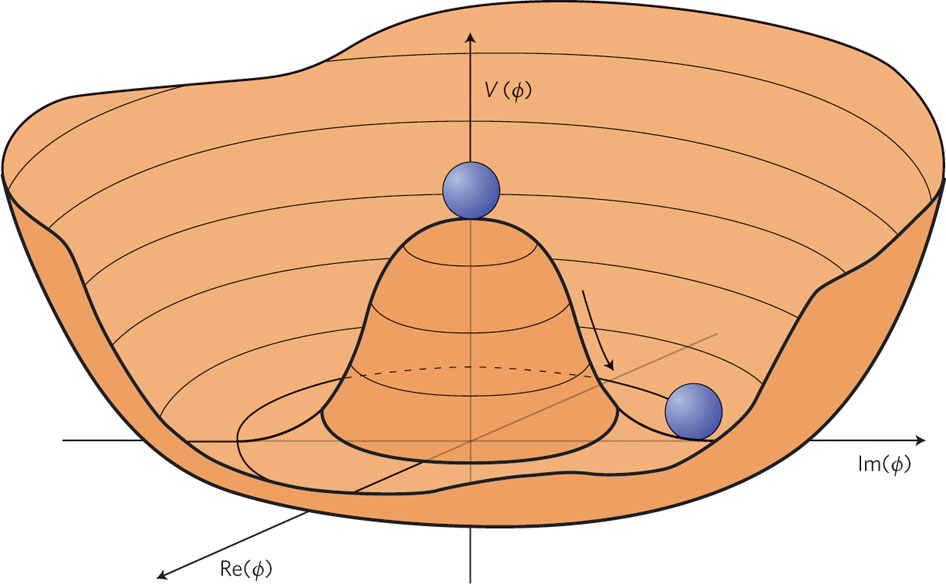
\includegraphics[width=0.7\textwidth]{nphys1874-f1.jpg}
  \caption{ The Higgs potential, $V(\phi)$, in the form of a 'Mexican hat',
leads to spontaneous symmetry breaking, from \cite{}}
  \label{fig:higgspot}
\end{figure}

A plot of the Higgs potential with $\mu^{2}<0$ is shown in
\FigureRef{fig:higgspot}. It is unstable to small perturbations, and will fall
to a lower energy state. /todo{reread}
As the ground state does not have the same symmetry as the Lagrangian, by
selecting a minima the symmetry has become broken. An example choice of minima
could be
\begin{equation}
\phi_{1} = \phi_{2} = \phi_{4} = 0
\end{equation}
and
\begin{equation}
\phi_{3} = \frac{-\mu^{2}}{\lambda} \equiv v^{2}
\end{equation}
This choice is motivated to ensure $U(1)_{EM}$ symmetry remains unbroken and
that the photon is massless.
Substituting this vacuum expectation value
\begin{equation}
\phi_{0} = \frac{1}{\sqrt{2}}\left(\begin{matrix}0\\v\end{matrix}\right)
\end{equation}
in to the Lagrangian, and using \EquationRef{eq:wgauge} and
\EquationRef{eq:bgauge}, additional terms are found,
\begin{equation}
\left(\frac{vg}{2}\right)^{2} W^{+}_{\mu} W^{- \mu}, 
\left(\frac{vg}{2}\right)^{2} \frac{1}{2\cos\theta_{W}} Z_{\mu} Z^{\mu}
\end{equation}
which appear to be mass terms for the gauge bosons.
The masses of the gauge bosons can be written as 
\begin{equation}
M_{W} = \frac{gv}{2}, 
M_{Z} = \frac{gv}{2\cos\theta_{W}}
\end{equation}
As there is no mass term for the photon (for example $A_{\mu}A^{\mu}$), it remains massless.

Another feature of the Higgs mecahnism, is that it also provides a way to
introduce mass terms for the fermions in a gauge invariant way via the Yukawa
coupling between the leptons with the Higgs field. The Lagrangian for this
interaction can be written as. 
\begin{equation}
\mathcal{L}_{yakawa} = -G_{f}\bar{L}\phi R + h.c.
\end{equation}
where $G_{f}$ is the coupling to the Higgs field known as the Yukawa coupling
\begin{equation}
-G_{f} = \frac{\sqrt{2}m_{f}}{v}
\end{equation}
which is proportional to the mass of the fermion. 

\subsection{QCD}
The final piece of the puzzle is the strong interaction, described by quantum
chromodynamics. 
Quantum chromodynamics follows from similar reasoning to the QED case, but with
the $U(1)$ symmetry group replaced with the SU(3) symmetry group of
transformations on the quark colour fields.

The local gauage phase transformation becomes

\begin{equation}
q(x) \to e^{i\alpha_a(x)T_a} q(x)
\end{equation}

Which breaks the invariance of the Lagrangian. Again this is overcome by
introducing the covariant derivative

\begin{equation}
D_{\mu} \equiv \partial_{\mu} + i g T_{a} G_{\mu}^{a}
\end{equation}

Where eight gauge fields have been introduced, instead of the single field in
QED.
The gauge fields transform as 
\begin{equation}
 G_{\mu}^{a} \to G_{\mu}^{a} 
-\frac{1}{g}\partial_{\mu}\alpha_{a}]
-f_{abc}\alpha_{b}G^{c}_{\mu}
\end{equation}
Where the additional term is to produce a gauge invariant Lagrangian due to the
non-Abelian gauge transformation.

The final Lagrangian for QCD can now be written.
\begin{equation}
\mathcal{L} = 
\bar{q}(i\gamma^{\mu}\partial_{\mu} - m)q -
g \bar{q} \gamma^{\mu} G_{\mu}^{a} - 
\frac{1}{4} G_{\mu\nu}^{a} G^{\mu\nu}_{a}
\end{equation}

where the field strength tensor $G^{\mu\nu}_{a}$ is given by:
\begin{equation}
G^{\mu\nu}_{a} 
= \partial{\mu} G^{a}_{\nu}
- \partial{\nu} G^{a}_{\mu}
-g f_{abc} G^{b}_{\mu} G^{c}_{\nu}
\end{equation}

In a simuilar way to QED, the Lagrangian for interacting coloured quarks, $q$, and
vector gluons, $G_{\mu}$, result from the simple erquirement of local colour
phase invariance of the quark fields. Unlike the QED case, eight gauge fields
are needed due to the three quark colour fields.  Similar to QED, the gluons are
required to  be massless.

The field strength tensor, $G^{\mu\nu}_{a}$, introduces terms that are cubic and
quadratic in $G$. These represent three and four vertex gluon interactions that
are a results of the non abelian nature of the $SU(3)$ group.

